\chapter{Variables and Computations}\label{chp:expressions}
\epigraph{Beauty is variable, ugliness is constant.}{Douglas Horton}

\emph{Useful} programs evolve over time. They compute some result or react to user input. To realize such dynamicity, C allows the existens of \emph{variables}, \ie stored information that can change over time. In this section we'll learn how to create and use variables and some of the \enquote{behind the scenes}, \ie what happens in memory when we use them.

\section{Memory Structure}
Imagine the memory as a long chain of enumerated cells. Each cell holds one byte's worth of information, \ie eight bits. These cells can never be empty; there's always \emph{some} information stored in them, albeit possibly nonsensical or useless. If we want to make use of this structure, someone or something will have to keep track of which cells hold which pieces of information, and how to interpret them.

Luckily, most of this bookkeeping is done automatically by the compiler; to properly utilize its features, however, we need to clarify some names.

Within the cells, we find \emph{values}. As mentioned, they are, a priori, pure bitpatterns with no inherent meaning. Provided we know \emph{what sort of information} they encode, we can make sense of these bitpatterns.

The question \emph{what sort of information} is contained in a cell is called \emph{data type}. The data type is a name for both, the method of interpretation of the raw data in the cells, as well as the \emph{number of bytes per unit of information}. From the previous chapter, you remember how to interpret bit patterns as signed integers; to do so, you also need to know how many bytes to consider in your interpretation. A \emph{32bit signed integer} is thus a data type.

The value we are looking for is in one of the enumerated cells. The \enquote{number of the cell} in which a given value is stored is its \emph{address}. An address itself can be stored as some unsigned integer. Adresses often are expressed as \emph{hexadecimal numbers}. That means, the number is written in base 16. You'll not only find the digits 0..9, but also A, B, ..., F (or, sometimes, the lower case letters a .. f). The digit 'A' then has the decimal value 10, 'B' is 11 and so on. The transformation back into base ten works just like described in section \ref{sec:BinaryNumbers}. To clarify that a number is given in hexadecimal, it often carries the prefix \texttt{0x}. More often than not, the exact value of addresses is of little importance; if you ever see hexadecimal numbers, simply know that they are just another way of writing normal decimal numbers.

As humans, we prefer symbols over addresses. \emph{The value of cell 238} doesn't tell a lot about its content or what it means. In contrast, \emph{the value of \texttt{nameOfPlayer1}} clearly signifies some textual information. We call \texttt{nameOfPlayer1} a \emph{symbol}. It is a stand-in for the address of the cell(s), in which the name of player 1 can be found. The compiler \emph{binds} the symbols we as humans choose to the addresses in memory.

\begin{defbox}[Memory Picture]
\begin{center}
\begin{tikzpicture}
  [
    cell/.style={text width=8mm,
      text height=4mm, draw=black, inner sep=1mm},
    ld/.style={draw=blue,shorten >=2pt,->}
  ]
  \node (c1) at (0,0) [cell] {\ttfamily 99};
  \node (c2) at (1,0) [cell] {\ttfamily 1};
  \node (c3) at (2,0) [cell] {\ttfamily 255};
  \node (c4) at (3,0) [cell] {\ttfamily 0};
  \node (c5) at (4,0) [cell] {\ttfamily 80};
  \node (c6) at (5,0) [cell] {\ttfamily ...};

  \node (labelMem) at (8,  1) {Symbols in our Code};
  \node (labelMem) at (8,  0) {Values in memory};
  \node (labelMem) at (8, -1) {Addresses};

  \node (a1) [below=2mm of c1]            {\tiny 0x27ff};
  \node (a2) [below=2mm of c2, color=red] {\tiny 0x2800};
  \node (a3) [below=2mm of c3]            {\tiny 0x2801};
  \node (a4) [below=2mm of c4]            {\tiny 0x2802};
  \node (a5) [below=2mm of c5]            {\tiny 0x2803};
  \node (a6) [below=2mm of c6]            {\tiny 0x2804};

  \node (ptr) [below=8mm of c1] {\scriptsize Address of \texttt{x}};
  \node (vc2) [above=6mm of c1] {\scriptsize Variable \texttt{x}};
  \node (vc0) [above=2mm of c1] {\scriptsize Variable \texttt{y}};

  \draw [ld] (ptr.east) .. controls +(0.3,0) .. (a2.south);
  \draw [ld] (vc0.east) .. controls +(0.4,0) .. (c2.north);
  \draw [ld] (vc2.east) .. controls +(2.4,0) .. (c4.north);
\end{tikzpicture}
\end{center}
\captionof{figure}{Variables in memory} \label{fig:memoryStructureBasic}
\end{defbox}

\begin{plusbox}[Powers of two in computing and why we use hexadecimal]
Everything in the world of computers is build around powers of two. There are 16bit-, 32bit- and 64bit operating systems, USB sticks with 2, 4, 8 or 16 GB and even your screen might be 1024, 2048 or 4096 pixels wide. This is no coincidence. Since everything boils down to collections of bits, powers of two are built into the very basis of our computation technology.

One nice aspect of hexadecimal numbers is that they \emph{align nicely} with binary numbers. I.\;e. round numbers in binary (numbers with lots of zeros) will also look like round numbers in hexadecimal (since 16 is also a power of two). The binary number $1000~ 0000_2$ translates to the decimal $128_{10}$ and to the hexadecimal $80_{16}$. The binary number $1111~ 0000~ 1100~ 0000_2$ is $F0C0_{16}$ in hexadecimal. Note also how each group of four binary digits corresponds to one hexadecimal digit. It is fortunately rare that we really have to deal with bit patterns directly; but when we have to do, being working with its hexadecimal representation is usually much more convenient than dealing with its binary or decimal form.

Powers of two appear so frequently, that some computer technicials expirience them as round numbers, regardless of their base representation. For example, Randall Munroe, author of the famous webcomic \href{https://www.xkcd.com/}{xkcd} celebrated his one thousandth strip with this comic:
\begin{center}
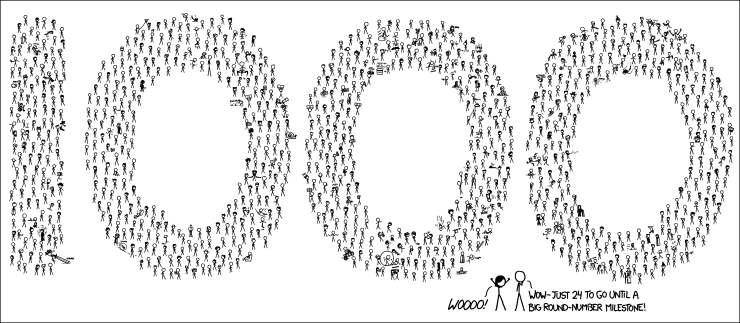
\includegraphics[width=.9\linewidth]{./gfx/xkcd-1000}
\end{center}
\captionof{figure}
	[Decimal and binary round numbers]
	{Decimal and binary round numbers. Source: \url{https://www.xkcd.com/1000/}}
\end{plusbox}

\section{Declaring Variables} \label{sec:DeclareVars}
To use variables in our code, we first have to \emph{declare} them. That means we have to tell the compiler that we want a variable and what kind of variable this should be. We do that with a statement of the form:
\begin{codebox}[Syntax: Declaring variables]
\texttt{dataType variableName;}
\end{codebox}

\texttt{dataType} stands for one of several registered keywords of the C programming language. Section \ref{sec:Datatypes} in the appendix lists all predefined data types. For the most part, we can limit ourselves to using one of these three:
\begin{center}
\newcolumntype{T}{>{\centering\ttfamily\arraybackslash}m{.2\linewidth}}
\newcolumntype{U}{>{\centering \arraybackslash}        p{.3\linewidth}}

\rowcolors{1}{white}{tabhighlight}
\begin{tabularx}
	{.5505\linewidth}
	{TU}
\toprule[1.5pt]
	\textbf{\textrm{data type}} & \textbf{use} \tabcrlf
	int                         & integers \\
	double                      & floating point numbers \\
	char                        & characters\footnote{
		\enquote{Character} means any one symbol, like \emph{A}, \emph{B}, \emph{C}, ... \emph{0}, \emph{1}, ..., \emph{!}, \emph{"}, etc. However, you've already encountered the fact that all of these
		symbols can be substituted for a number -- their ASCII code. So, the datatype \inC{char} actually is just a form of an integer that exactly takes up one byte and thus can 
		represent numbers from -128 through 127. They are most often meant to represent symbols in a longer text.
	} \\
\bottomrule[1.5pt]
\end{tabularx}
\captionof{table}{The most commonly used data types in C}
\end{center}

\texttt{variableName} is an arbitrary identifyer we can choose, like \texttt{nameOfPlayer1}. It must abide to these rules: \vspace{-9pt}
\begin{itemize}
\setlength\itemsep{0pt}
\item Must only comprise of the characters \texttt{a..z}, \texttt{A..Z}, \texttt{0..9} or \texttt{\_}
\item The first character must not be a digit
\item Must have at most 40 characters
\item Must be unique (there may not be two symbols with the same name in the same section. For example, it is not allowed to have a variable named \texttt{main} 
	since there has to be a function with that name\footnote{\emph{Technically}, there is a way around that... practically... \url{https://xkcd.com/1475/}}.)
\end{itemize}
\vspace{-8pt}

The language C is \emph{case sensitive}, \ie there is a difference between \texttt{nameOfPlayer1} and \texttt{NameOfPlayer1}. By convention, variable names start with a lower case letter. If a variable comprises of several human language words (like \texttt{nameOfPlayer1}) one often applies \enquote{camel case}, \ie begin each new word in the symbol with an upper case letter (except for the first one). An alternative is \enquote{snake case}, where the individual words are separated by underscores (\texttt{name\_of\_player\_1}). Which of the two conventions you pick is up to you; again I only advise you to be consistent in your choice (otherwise you'll have a hard time remembering whether you spelled it \texttt{paragraph\_index} or \texttt{paragraphIndex}.)

\begin{hintbox}[Good names]
A common \enquote{mistake} among beginners is to use inexpressive names such as \texttt{x}, \texttt{y}, \texttt{a}, ... While this is no problem for the compiler (note the quotation marks around \enquote{mistake}), it makes codes harder to write, maintain and debug. Programming becomes quite complex very soon, and the last thing we want is loosing track of whether \texttt{a} is the total score or which is the meaning behind the variable \texttt{b}.

Instead, be as descriptive as possible when giving names. A guideline to follow is \emph{good code should read like prose text}. That certainly is only possible if the variables are named after human concepts like \texttt{repetitions}, \texttt{message}, \texttt{velocity\_x}, ...
\end{hintbox}

\begin{hintbox}[Efficiency and accuracy through data types]
In principle, you could use the data type \inC{double} for all your numbers, since any integer can be converted into a floating point value. However, operations involving integers are usually faster that such involving floating point numbers. The memory consumption for an \inC{int} also is (usually -- see appendix table \ref{tab:DatatypesStd}) only half as much as that of a \inC{double}. The most important reason to use integers over floating point values is, however, that the latter always accumulate rounding errors with each computation. Only integer math is guaranteed to be exact (unless there is an overflow, \ie the computed number becomes too big to be stored in an \inC{int} variable).
\end{hintbox}

A \emph{declaration} (\ie a line like \inC{int number;}) does two things: it \emph{reserves memory} (\ie it picks a number of consecutive cells in memory and tells the operating system that they are used now) and \emph{binds the memory to the variable name} (\ie the compiler knows that \texttt{variableName} should refer to the content of the reserved memory cells).

Multiple variables \emph{of the same type} can be declared in a single statement\footnote{However, this programming style is sometimes discouraged.}. To do so, we list them separated by commas. A valid declaration of variables could thus look like this:
\begin{codebox}[declarations.c]
\begin{minted}[linenos]{c}
int main () {
   int    count;
   double positionX, positionY;
}
\end{minted}
\captionof{code}{Declaration of variables} \label{code:declaringVars}
\end{codebox}

You may have noticed the similarity between the definition of the variable \texttt{count} and the function \texttt{main}. That is no coincidence! From the viewpoint of the compiler, the function \texttt{main} is a set of instructions to compute an \inC{int}. We'll learn more about this in chapters \ref{chp:funcs} and \ref{chp:OS-Link}.

\begin{warnbox}[No duplicates or redeclarations]
Variables that have been declared once cannot be declared again. In the following example, there are multiple \emph{forbidden} lines:
\vspace{3pt}

\begin{codebox}[redeclaration.c]
\begin{minted}[linenos]{c}
int main () {
    int x;
    double x;
    int x;
}
\end{minted}
\captionof{code}{Attempts of redeclaration} \label{code:redeclarations}
\end{codebox}
The problems are: \vspace{-6pt}
\begin{itemize}
\setlength\itemsep{-0pt}
\item Line 3: the variable \texttt{x} already exists (line 2) and cannot be re-typed to \inC{double}.
\item Line 4: again, the variable \texttt{x} already exists; even repeating an identical declaration is not allowed.
\end{itemize}

Consequently, trying to compile code \ref{code:redeclarations} will result in error messages:
\begin{cmdbox}[Error messages produced by code redeclarations.c]
\begin{minted}{text}
redeclaration.c: In function ‘main’:
redeclaration.c:3:12: error: conflicting types for ‘x’; have ‘double’
    3 |     double x;
      |            ^
redeclaration.c:2:9: note: previous declaration of ‘x’ with type ‘int’
    2 |     int x;
      |         ^
redeclaration.c:4:9: error: conflicting types for ‘x’; have ‘int’
    4 |     int x;
      |         ^
redeclaration.c:3:12: note: previous declaration of ‘x’ with type
    ‘double’
    3 |     double x;
\end{minted}
\end{cmdbox}
\end{warnbox}

\begin{warnbox}[Avoid global variables]
Note that the declaration of the variables \texttt{count}, \texttt{positionX} and \texttt{positionY} is \emph{within} the function \texttt{main}. We \emph{could} also define them outside of \texttt{main}; but this would potentially lead to a lot of trouble. We'll discuss the implications of that placement in chapter \ref{chp:funcs}. For now, just stick to the rule:

Anything that is not an \texttt{\#include} line must be \emph{within} the braces that belong to \inC{int main}.
\end{warnbox}

\section{Assignments} \label{sec:valueAssignment}
We can assign values to our varibles with the \emph{operator} \texttt{=}:
\begin{codebox}[assignments.c]
\begin{minted}[linenos]{c}
int main () {
    int    count;
    double positionX, positionY;

    count = 7;
    count = 8;

    positionX = 4.3;
    positionY = 5.0;
}
\end{minted}
\captionof{code}{Assigning values to variables} \label{code:simpleAssignment}
\end{codebox}

In this, line 5 makes it so that \texttt{count} stores the value \inC{7}. The subsequent line 6 overwrites this value and assigns \inC{8} to \texttt{count}.

The lines 8 and 9 also assign values to the two previously defined \inC{double} variables. Note that we use a dot as a decimal separator\footnote{In some parts of the world, using a comma as a decimal separator. One example for this is Germany, my humble country of origin.}. Note also that \texttt{positionY} is assigned the value \inC{5.0} (as opposed to simply \inC{5}): the data types of variable and assigned value match, \ie they're both floating point values. In chapter \ref{chp:casting} we'll discuss what happens if you don't abide by this rule (and when this is possible in the first place).

\begin{hintbox}[Order of statements]
(Unlike humans), the computer can only \enquote{read} code from top to bottom. We've heard this before when we discussed the \texttt{\#include} preprocessor directive, and of course it affects all code equally. In particular, this means that variables have to be declared before they are used. In example \ref{code:simpleAssignment}, if moved line 2 (declaration of \texttt{count}) to line 7 (after writing \texttt{count}), compilation would fail and we'd see the error message:

\begin{cmdbox}[Error message: undeclared identifier]
\begin{minted}{text}
assignments.c: In function ‘main’:
assignments.c:5:5: error: ‘count’ undeclared (first use in this function)
    2 |     count = 7;
      |     ^~~~~
assignments.c:5:5: note: each undeclared identifier is reported only once 
    for each function it appears in
\end{minted}
\end{cmdbox}

The last line (\emph{each undeclared identifier is reported only once for each function it appears in}) means that, albeit line 6 (\texttt{count = 8}) is equally faulty without declaration of the symbol \texttt{count}, it is not reported by the compiler because it has already uttered an error message related to the symbol \texttt{count}.
\end{hintbox}
%
\begin{hintbox}[]
A real life counterpart of this scenario would be this: I tell you to write the number 7 on \emph{the paper}. My desk is cluttered with different pieces of paper, so you would have no idea where I wanted you to put that note to. When I later tell you that \emph{the paper} means the blue post it on the left, it's already too late: you've written the number to some other piece of paper, because as a human, you can proactively make decisions. A computer does not have the capacity to make decisions of its own (remember our mantra), and hence, the only thing it can do is complain by means of an error message.
\end{hintbox}


\subsection{Combined Declaration and Assignment} \label{sec:valueAssignment}
Declaration and assignment can be done in a single statement:
\begin{codebox}[combinedAssignments.c]
\begin{minted}[linenos]{c}
int main () {
    int    count = 8;
    double positionX = 4.3,
           positionY = 5.0;
}
\end{minted}
\captionof{code}{Combined declaration and assignment} \label{code:combinedAssignment}
\end{codebox}

The final \emph{state} (\ie totality of values in memory) after running code \ref{code:combinedAssignment} is the same as that after executing code \ref{code:simpleAssignment}. Note how line 3 and 4 form a \emph{single statement}: line 3 ends in a comma, which does not end the statement. Only the semicolon in line 4 ends the declartion of \inC{double} variables. The statement could also be compressed into one line of code: \texttt{double positionX = 4.3, positionY = 5.0;}

\begin{hintbox}[Uninitialized variables]
When declaring variables (like in code \ref{code:declaringVars}), the compiler only \emph{reserves} memory for the variable, but does not write any value into the reserved cell(s). However, there is no such thing as an empty memory cell; each byte in memory always holds some bitpattern. Directly after declaration, this can be anything: maybe the same memory cell has been used previously by another program and still holds a character of a text the program displayed. Essentially, the value a variable has after declaration is random!

If your program \emph{reads} an uninitialized value \ie does anything with the variable other than assigning it a value, the result will be \emph{undefined behaviour}. Results of this can be benign (\eg  strange outputs on the console) bad (\eg crash of your program) or outright harmful (\eg overwriting files), depending on what you do with the uninitialized variables. More often than not, it is not always obvious that an uninitialized variable causes trouble; there could be a range of values of the uninitialized variable for which the behaviour of the program looks fine, and only certain values cause glitches, crashes or damage. Still, it is a condition we should avoid at all cost.

For that reason, I strongly advise you to \emph{always} initialize your variables with some default value, \ie to always use the combined declaration and assignment syntax. If you are not sure which default value is the best for your specific problem, simply put in \texttt{0}. It is easier to debug problems caused by one known value than such caused by a completely random factor.
\end{hintbox}


\section{Using Variables in Computations}\label{sec:OperatorsArithmetic}
The point of computers is to compute\citationneeded[https://xkcd.com/703/]! Computations have an input and an output. This input can be \emph{constants} (such as \inC{5}) or variables. The output needs to be stored somewhere, too, so again we'll see the use of variables here.

Computations are written as \enquote{normal} expressions as we know them from our human every day experience; for example \inC{5 + 3} instructs the computer to sum up the constants \inC{5} and \inC{3}. The result of this \emph{expression} can then be stored in a variable with an assignment, like we've seen them before. This works with both, the simple assignment and the combined declaration/assignment:
\begin{codebox}[computations.c]
\begin{minted}[linenos]{c}
int main () {
    int count = 5 + 3;
    int nextCount;    
    nextCount = (count - 3) * 7;
}
\end{minted}
\captionof{code}{Computations with variables} \label{code:simpleComputations}
\end{codebox}
In this, the value of \texttt{nextCount} will be \inC{35}.

Valid \emph{operators} in C are:
{
\newcolumntype{N}{>{         \centering\arraybackslash} p{.25\linewidth}}
\newcolumntype{R}{>{\ttfamily\centering\arraybackslash} p{.15\linewidth}}
\begin{center}
\rowcolors{1}{tabhighlight}{white}
\begin{tabularx}
	{.907\linewidth}
	{NR|NR}
\toprule[1.5pt]

    \textbf{Operation}       & \textrm{\textbf{Operator}}  &  \textbf{Operation}                       & \textrm{\textbf{Operator}}
\tabcrlf
    Addition                 & +                           &  Multiplication                           & * \\
    Subtraction              & -                           &  Division                                 & / \\
    Negation ($x \thus -x$)  & -                           &  Remainder of Division (\enquote{Modulo}) & \%\\

\bottomrule[1.5pt]
\end{tabularx}
\end{center}
\captionof{table}{Arithmetic operators in C}\label{tab:OperatorsArithmetic}
}

As you've seen in example \ref{code:simpleComputations}, you can also use parentheses to affect the order of evaluation. Precedence of operations (multiplication is evaluated before addition) is also respected. Later in this course, we'll learn about other operations; all of them and their precedence are summarized in the appendix in table \ref{tab:OperatorPrecedence}. Note that there is no exponentiation operator; we'll see in chapter \ref{chp:maths} how in C we can compute powers nonetheless.

\begin{hintbox}[Expressions vs. statements vs. declarations]
In the programming world, we make a distinction between \emph{expressions}, \emph{statements} and \emph{declarations}.

\begin{itemize}
\setlength\itemsep{0pt}
\item An \emph{expression} is anything that can be \emph{evaluated}, \ie condensed into a single value. Examples for statements are \inC{5 + 3} (evaluated to \inC{8}) 
	or \inC{count - 3} (evaluation depends on the current value of the variable \texttt{count}).
\item A \emph{statement}, on the other hand, is one single complete line of code that changes the \emph{state of the machine}, \ie changes some values in memory\footnote{well... actually,
	there also are statements that do nothing at all... but saying a statement changes the state of the machine will give you the correct intuition, at the very least.}.
	For example \inC{printf("hello world\n");} is a statement (it changes the video memory that is used to show the output on screen).
\item \emph{Declarations} look a lot like statements, but do not not change the \emph{content} of memory, but only introduce symbols.
	The line \inC{int count;} is a declaration: it merely informes the compiler that some memory has to be reserved, but the contents of the memory are not changed.
\end{itemize}

Preprocessor directives are considered a different thing alltogether, since they are replaced by \enquote{proper} C code before compilation. We've only encountered the directive \texttt{\#include} so far, which pastes the content of another file into our code before compilation. Other directives have similar effects in that they only generate C code which then might be be a declaration of symbols, an executable statement or an evaluatable expression.

For very technical reasons, a line like \inC{int count = 8;} is not considered a statement, but a \emph{declaration with initialization}. One rationale behind this is that such lines cannot be executed several times in a row: once a symbol has been introduced, it exists. Remember that \emph{redeclarations} (\ie binding the symbol to a new location in memory) is forbidden (cf. code \ref{code:redeclarations}).

To muddy the waters, in chapter \ref{chp:funcs} we'll see that there are statements that are also expressions at the same time. You don't need to worry too much about these differences for now; but be aware that they exist when discussing with fellow programmers.
\end{hintbox}

Assignments are always made from the right to the left. I.\;e. on the right hand side of the equals sign, there's an expression that will be stored in the variable on the left hand side\footnote{In section \ref{sec:Pointer}, we'll see that the left hand side of an assignment can also be an expression; however, this expression has to evaluate to a variable, as opposed to a value. We'll see soon enough what that means.}.

\begin{tcbraster}[raster columns=2,
                  raster equal height,
                  nobeforeafter,
                  raster column skip=0.2cm]
\begin{codebox}[Correct order of expression and variable]
\inC{result = 2 + 2;}
\end{codebox}
%
\begin{warnbox}[Wrong order of expression and variable]
\inC{2 + 2 = result;}
\end{warnbox}
\end{tcbraster}

\subsection{Divisions}
When dividing two numbers, we need to be extra careful. For a computer there are \emph{two kinds of division}: \emph{integer division} and \emph{floating point division}. The names already give away the difference -- the result data type of the two operations is different. While the floating point division produces the result we as humans would consider correct, the integer division might round down to the nearest integer. Both operations are invoked by the same symbol (the division operator \texttt{/}). Integer division takes place when both operands (dividend and divisor) are \inC{int}-like types (appendix section \ref{sec:Datatypes} lists some other data types that behave like \inC{int}s in this respect). If either operand or both operands are floating point numbers, the floating point division will be executed.

\begin{codebox}[divisions.c]
\begin{minted}[linenos]{c}
int main () {
    int    dividend_int    = 3;
    double dividend_double = 3.0;
    
    int    divisor_int    = 2;
    double divisor_double = 2.0;

    int    result_1 = dividend_int    / divisor_int;
    
    double result_2 = dividend_double / divisor_double;
    double result_3 = dividend_int    / divisor_double;
    double result_4 = dividend_double / divisor_int;

    int    result_5 = dividend_double / divisor_double;
}
\end{minted}
\captionof{code}{Integer and floating point divisions} \label{code:divisions}
\end{codebox}

In listing \ref{code:divisions} we'll find the following results:\vspace{-9pt}
\begin{itemize}
\setlength\itemsep{-6pt}
\item \texttt{result\_1} will be computed from an integer division, since both operands are integers. Hence the \enquote{mathematically correct} result $1.5$ will be rounded down to 
	the nearest integer, which is \inC{1}.
\item All of \texttt{result\_2} through \texttt{result\_4} trigger floating point division, since at least one operand is a \inC{double}. Hence, these three variables all store the 
	value \inC{1.5}.
\item \texttt{result\_5} is of type \inC{int}. Although the computation itself is done as a floating point division and produces the intermediate result \inC{1.5}, the computer cannot 
	store a \inC{double} result in an \inC{int} variable. Instead, this intermediate result is again rounded to \inC{1}. More on this in chapter \ref{chp:casting}.
\end{itemize}


\section{Formatted Output}
It's nice that we can make the computer do computations for us. But up to now, all we know is that the results are \emph{somewhere in memory}, which is not very useful for us as humans. Luckily, the command \texttt{printf} can do more than print constant strings. It actually can also print the value of variables. For that, we use a new or extended syntax:

\begin{codebox}[Syntax: printf]
printf(formatString, commaSeparetedListOfExpressions);
\end{codebox}

In this, ...\vspace{-12pt}
\begin{itemize}
\setlength\itemsep{0pt}
\item \texttt{formatString} is a string (\ie text between \texttt{"}double quotes\texttt{"}) that tells the computer what to print where. Essentially, it is regular text with special
	characters that act as placeholders; the value of one or more variables will be substituted for these placeholders. Placeholders begin with a percent sign (\texttt{\%}) and will be
	explained in more detail below.
\item \texttt{commaSeparetedListOfExpressions} is, well, a comma separated list of expressions. That means, it can be one or several variables, constants or entire computations. This list 
	may also be empty, \ie it can be ommitted.
\end{itemize}

By know we well know the line \inC{printf("Hello World!\n");}. In this, \inC{"Hello World!\n"} is the format string; it simply contains no placeholders and is consequently printed as-is.\\
The \texttt{commaSeparetedListOfExpressions} is ommitted in this form, \ie there are no expressions to fill in.

An example with a \emph{nonempty} list of expressions is the following:
\begin{codebox}[formatStrings.c]
\begin{minted}[linenos]{c}
int main () {
    int data = 1;
    printf("data = %d, constant = %d\n", data, 90 + 9);
}
\end{minted}
\captionof{code}{A simple format string} \label{code:simpleFormatString}
\end{codebox}

\begin{cmdbox}[Output: formatStrings.c]
data = 1, constant = 99
\end{cmdbox}

In this listing \ref{code:simpleFormatString}, we see two percent signs in the format string, which tells the computer that it has to fill in two values. Consequently, after the format string, there are two expressions: \texttt{data} and \inC{90 + 9}. So, a string representation of the current value of \texttt{data} (which is \inC{1}) is computed and replaces the first percent sign; likewise, a string representation of the constant value \inC{99} replaces the second placeholder.

So what does the \texttt{d} after the percent signs mean? As we've seen before, there are numerous ways, the same information can be encoded, both in binary and as human-readable text. The computer needs to know both, what kind of bitpattern to expect and what kind of text to produce. In this case, \texttt{\%d} stands for \emph{expect an \inC{int} and render it as a decimal number}.

In the appendix, tables \ref{tab:FormatOutNum} and \ref{tab:FormatOutSpc} you'll find an entire zoo of format codes that you may use in your format strings. Most of the time, you'll need only these four symbols:
{
\newcolumntype{N}{>{         \centering\arraybackslash} p{.25\linewidth}}
\newcolumntype{R}{>{\ttfamily\centering\arraybackslash} p{.15\linewidth}}
\begin{center}
\rowcolors{1}{tabhighlight}{white}
\begin{tabularx}
	{.907\linewidth}
	{NR|NR}
\toprule[1.5pt]

    \textbf{Data}     & \textrm{\textbf{Format Code}}  &  \textbf{Data}         & \textrm{\textbf{Format Code}}
\tabcrlf
    \texttt{int}egers & \%d                            &  single characters     & \%c \\
    \texttt{double}s  & \%lf                           &  strings of characters & \%s \\

\bottomrule[1.5pt]
\end{tabularx}
\end{center}
\captionof{table}{Most common format string elements in C}\label{tab:formatStringCommon}
}

\begin{hintbox}[Literal Percent Sign]
If you need to print a percent sign, you can do so by putting a double percent sign in your format string:
\mint{c}{printf("The result is %lf%%.\n", result);}
will give you an output like:\\
\texttt{The result is 49.570000\%.}
\end{hintbox}

\begin{warnbox}[Matching Data Types]
Always make sure that the data types in the format string match the data types of the actual expressions! That is, if you type \texttt{\%d} in your format string, you had better provide an \inC{int} value for that place holder. Likewise, make sure the number of expressions and their order matches that of the placeholders. If you disregard this rule, ...
\begin{itemize}
\setlength\itemsep{0pt}
\item you'll get a compiler warning\footnote{only if you compile with the \texttt{-Wall} compiler option} (which is the nicer part of the outcome)
\item you'll find utter BS on screen.
\end{itemize}

\begin{tcbraster}[raster columns=2,
                  raster equal height,
                  nobeforeafter,
                  raster column skip=0.2cm]
\begin{warnbox}[nonmatchingFormat.c, leftupper=7mm]
\begin{minted}[linenos]{c}
#include <stdio.h>

int main () {
    int    integral = 1;
    double decimal  = 1.0;
    
    printf("%lf\n", integral);
    printf("%d\n", decimal);
}
\end{minted}
\captionof{code}{Format mismatch}
\end{warnbox}
%
\begin{cmdbox}[Output: nonmatchingFormat.c]
0.000000 \\
1100706464
\end{cmdbox}
\end{tcbraster}
%
\begin{cmdbox}[Compiler Warnings: nonmatchingFormat.c]
\begin{minted}{text}
nonmatchingFormat.c: In function ‘main’:
nonmatchingFormat.c:7:15: warning: format ‘%lf’ expects argument of type 
   ‘double’, but argument 2 has type ‘int’ [-Wformat=]
    7 |     printf("%lf\n", integral);
      |             ~~^     ~~~~~~~~
      |               |     |
      |               |     int
      |               double
      |             %d
nonmatchingFormat.c:8:14: warning: format ‘%d’ expects argument of type 
   ‘int’, but argument 2 has type ‘double’ [-Wformat=]
    8 |     printf("%d\n", decimal);
      |             ~^     ~~~~~~~
      |              |     |
      |              int   double
      |             %f
\end{minted}
\end{cmdbox}

Note how the compiler is really helpful here and highlights not only the line in which the error occured, but explicitly names the expected and given data types, as well as giving a recommendation which format string elements you should be using here.
\end{warnbox}

\begin{plusbox}[Undefined Behaviour]
When the data type in the format string does not match the data type of the expression, it is very difficult to understand \emph{exactly} why any given (certainly nonsensical) output is generated. In fact, even if one does understand the inner workings of the command \texttt{printf}, it isn't even possible to predict which numbers are written on screen. \emph{One mechanism} that messes up the output here is the following:

Remember that any piece of information is stored as a bit pattern of varying length. A \inC{double} value is a sequence of 64 bits, while an \inC{int} (usually) takes up 32 bits. A command like \texttt{printf("\%lf", ...);} consequently instructs the computer to read 64 bit from memory and interpret them as a double. Now, if we pass an \inC{int} here in the list of expressions, we provide too few information for the job. However, the computer ignores this fact; it simply starts reading bits from memory at a given starting point. We provided half of the data that are going to be read. But there are no empty cells: the computer continues reading behind the point where we put our data, and takes whatever information it finds there as part of a \inC{double} 
number.

You can imagine this like so:

You are a journalist for a local newspaper. You and your colleagues all submit your articles, which are printed in the newspaper. In this parable, your article corresponds to the expression you want to print; your colleagues articles stand for other processes on your computer that you do not control directly but that all use space somewhere in memory. The entirety of memory is the printed newspaper.

Now with the newspaper printed (the memory prepared), you tell a friend to read your article. Unfortunately, your friend is mentally challenged, so you have to tell him where to start, how long the article is, and which language it is written in. The \emph{where} information is contained in the expression list; the \emph{what and how long} is given in the format string. If you mistakenly tell your friend to read more than the length of your article, they will continue taking up words your colleagues have written and think that they belong to your article. Also, even if you tell them the correct length, they may not be able to make any sense of your work if you told them to expect the wrong language.

Both, length and language are contained in the format string specification: \texttt{\%lf} stands for 64 bits worth of information (length) and \inC{double} format (language).
\end{plusbox}

\subsection{Controling Length and Alignment of the Output}
By default, \texttt{printf} will write as many characters on screen as it takes to render the information stored in our variables. Sometimes, however, we want our output to have a nice tabular format. Compare these two outputs\footnote{Source: The CIA World Factbook, September 2022, \url{https://www.cia.gov/the-world-factbook/}}:
\begin{tcbraster}[raster columns=2,
                  raster equal height,
                  nobeforeafter,
                  raster column skip=0.2cm]
\begin{cmdbox}[Output 1: non-aligned]
\begin{minted}{text}
PERCENTAGE OF WIND POWER IN 2020:
Germany: 23.9%
France: 7.3%
Spain: 22.1%
United Kingdom: 25.2%
\end{minted}
\end{cmdbox}
%
\begin{cmdbox}[Output 2: aligned]
\begin{minted}{text}
PERCENTAGE OF WIND POWER IN 2020:
Germany             : 23.9%
France              :  7.3%
Spain               : 22.1%
United Kingdom      : 25.2%
\end{minted}
\end{cmdbox}
\end{tcbraster}

I think you will agree that the right hand side output looks nicer and allows for easier comparison and interpretation of the data by an end user. Of course we can achieve this look by putting an according number of white spaces into the format string in the \texttt{printf} statement:
\begin{codebox}[manuallyAlignedOutput.c]
\begin{minted}[linenos]{c}
...

double percentGermany = 23.9;
double percentFrance = 7.3;
double percentSpain = 22.1;
double percentUK = 25.2;

printf("%s             : %lf%%\n", "Germany", percentGermany);
printf("%s              :  %lf%%\n", "France", percentFrance);
printf("%s               : %lf%%\n", "Spain", percentSpain);
printf("%s      : %lf%%\n", "United Kingdom", percentUK);
\end{minted}
\captionof{code}{Manually aligned output}
\end{codebox}

But you will agree that this piece of code doesn't look very nice. Much worse, if we want to display the same table for a different year, we have to tediously re-align the output. Rather than that, we can leave the \emph{padding with whitespaces} to be done automatically by the inner workings of \texttt{printf}.

To do so, we can wedge additional information between the percent sign and the data type code. In the most simple case, this is an integer, specifying the \emph{field width} of the placeholder field:
\vspace{-9pt}
\mint{c}{printf("%20s: ...", "France");}
\vspace{-9pt}
instructs the computer to print a string (\texttt{\%s}) that is right aligned and 20 characters wide. If the actual string to be printed (in this case \inC{"France"}) is less than 20 characters wide, the rest is simply padded with white spaces. The resulting output hence is "\texttt{~~~~~~~~~~~~~~France: ...}"

To produce a left-aligned string, one can simply flip the sign of the width information:
\vspace{-9pt}
\mint{c}{printf("%20s: ...", "France");}
\vspace{-9pt}
will produce the output "\texttt{France~~~~~~~~~~~~~~: ...}"

The same modifier can also be applied to numbers:
\vspace{-9pt}
\mint{c}{printf("%20s: %10lf", "France", percentFrance);}
\vspace{-9pt}
results in the output "\texttt{France~~~~~~~~~~~~~~: ~7.300000\%}"

This is already enough to produce nice tabular output; but maybe you don't like the fact that floating point numbers will always be printed with 6 digits after the decimal point. To change this behaviour, we can add an additional \emph{precision modifier} to the format string\footnote{of course, this only works for \inC{double} and \inC{float} values, not for \inC{int}s, strings or other data types}. This means, you can add a dot and another integer in the format string, after the field width information:
\vspace{-9pt}
\mint{c}{printf("%20s: %4.1lf", "France", percentFrance);}
\vspace{-9pt}
produces "\texttt{France~~~~~~~~~~~~~~: ~7.3\%}"

Note that the \emph{field width} (in this case 4) counts the entire length of the output in characters, \emph{including the decimal point}. The format string \texttt{\%4.1f} instructs the computer to produce an output that is \emph{at least} 4 characters wide, of which one character will be the decimal point and one will be the digit after the decimal point. So there will be two digits left of the decimal point. Also remember that, if you're dealing with negative values, you might need to reserve one extra character.

The complete code to produce the tabular output from the beginning of this section is thus:
\begin{codebox}[autoalignedOutput.c]
\begin{minted}[linenos]{c}
#include <stdio.h>

int main () {
    double percentGermany = 23.9;
    double percentFrance = 7.3;
    double percentSpain = 22.1;
    double percentUK = 25.2;
\end{minted}
\end{codebox}
%
\begin{codebox}[]
\begin{minted}[linenos, firstnumber=last]{c}
    printf("PERCENTAGE OF WIND POWER IN 2020:");
    printf("%-20s: %5.1lf\n", "Germany", percentGermany);
    printf("%-20s: %5.1lf\n", "France", percentFrance);
    printf("%-20s: %5.1lf\n", "Spain", percentSpain);
    printf("%-20s: %5.1lf\n", "United Kingdom", percentUK);
}
\end{minted}
\captionof{code}{Automatically aligned output}
\end{codebox}

Note that the field width information only gives the \emph{minimal} width; if a value is too large, \texttt{printf} will simply allocate more space for the output:
\begin{tcbraster}[raster columns=2,
                  raster equal height,
                  nobeforeafter,
                  raster column skip=0.2cm]
\begin{codebox}[oversizedOutput.c]
\begin{minted}[linenos]{c}
#include <stdio.h>

int main () {
    int small = 1, big = 1000000;

    printf("small: |%3d|\n", small);
    printf("big  : |%3d|\n", big);
}
\end{minted}
\captionof{code}{Value too big for format specification}
\end{codebox}
%
\begin{cmdbox}[Output 2: oversizedOutput.c]
\begin{minted}{text}
small: |  1|
big  : |1000000|
\end{minted}
\end{cmdbox}
\end{tcbraster}

You will find a detailled list of allowed format codes and modifiers in the appendix, tables \ref{tab:FormatStringBase} and \ref{tab:FormatStringModifiers}.

\section{Pointers}
Now that we've familiarized ourselves with the type system in C and also have tools to output results on screen, let's introduce a new kind of information:

In the beginning of this chapter, we've learned that all information in memory resides in enumerated cells; the numbers of the memory cells are now known to us as \emph{addresses}. Since addresses really are nothing other than numbers, we can store them in variables, \eg of type \inC{int}\footnote{or rather, of type \inC{long long int}. There are usually several gigabtyes worth of memory, so the number of a cell tends to be a very big number.}. However, knowing that a number is an address gives some extra context. There are operations that we can do with addresses that would make no sense with other numbers; and, vice versa, there are arithmetic operations that are considered not useful when dealing with addresses.

To reflect this special context, C has a dedicated data type for adresses, or rather: an entire family of data types. These types are called \emph{pointer types}, and the variables that belong to that type are called \emph{pointers}. We declare them \emph{almost} like normal variables; the only difference is an asterisk (\texttt{*}) after the type name:

\begin{codebox}[Syntax: Declaring pointer variables]
\texttt{baseDataType * variableName;}
\end{codebox}

\texttt{baseDataType} is any type name like \inC{int} or \inC{double}. The word \texttt{\emph{base}DataType} is meant to represent the idea, that this pointer stores the address of a value of type \texttt{baseDataType}. Since \inC{int*} (say: \emph{pointer to \inC{int}}) is a data type in its own right, \inC{int} is considered the base of the data type.

Like before, \texttt{variableName} is a new name conforming to the same rules as any other variable.

\begin{defbox}[Dissection of the statement]
Note that the asterisk is part of the type name. Declaring a pointer follows \emph{exactly the same syntax} as declaring any other variable.

\begin{center}
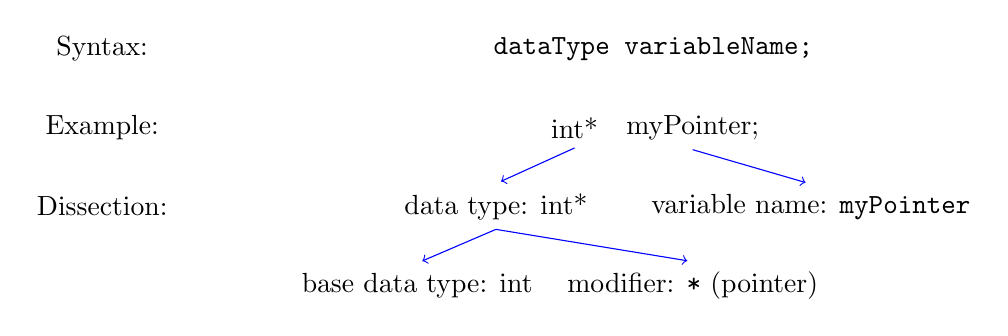
\begin{tikzpicture}
  [
    cell/.style={text width=8mm,
      text height=4mm, draw=black, inner sep=1mm},
    ld/.style={draw=blue,shorten >=2pt,->}
  ]
  
  \node (schemeGen) at (0,3) {Syntax:};
  \node (schemeXmp) at (0,2) {Example:};
  \node (schemeDis) at (0,1) {Dissection:};

  \node (declGen) at (7,3) {\texttt{dataType variableName;}};  
  \node (declType) at (6,2) {\inC{int*}};  
  \node (declName) at (7.5,2) {\inC{myPointer;}};  
  
  \node (dis1_1) at (5,1) {data type: \inC{int*}};
  \node (dis1_2) at (9,1) {variable name: \texttt{myPointer}};

  \node (dis2_1) at (4,0) {base data type: \inC{int}};
  \node (dis2_2) at (7.5,0) {modifier: \texttt{*} (pointer)};

  \draw [ld] (declType.south) -- (dis1_1.north);
  \draw [ld] (declName.south) -- (dis1_2.north);
  
  \draw [ld] (dis1_1.south) -- (dis2_1.north);
  \draw [ld] (dis1_1.south) -- (dis2_2.north);
\end{tikzpicture}
\end{center}
\captionof{figure}{Variables in memory} \label{fig:memoryStructureBasic}
\end{defbox}

\begin{plusbox}[Higher order Pointers]
Any data type can be used as a base data type. Pointer types, too, are data types. So you can also have pointers to pointers. This is only consequent: If some piece of information has an address and you store that address in memory, the address itself will have its own address.

Such handling of meta-information is not uncommon in C. It takes some time to get used to this abstraction, so we'll take it slowly. However, I think it does not hurt to be prepared to encounter an \inC{int**} before we get to the point where we need them.
\end{plusbox}

\subsection{Pointer Specific Operations}
Now that we have variables dedicated to storing addresses, we will first want to find suitable values to store in there. Of course, with pointers essentially being numbers, we could just pick any value that we fancy...

\begin{warnbox}[unguardedAddress.c, leftupper=7mm]
\begin{minted}[linenos]{c}
int main () {
    int* myPointer = 1000;
}
\end{minted}
\captionof{code}{An unguared address}
\end{warnbox}

... but who guarantees that no other programm on the computer is currently using this address\footnote{... the operating system, usually. However, there are still good reasons not to do this.}? Rather than randomly poking around in memory, we rather only refer to \emph{properly allocated memory} (memory that is explicitly reserved for use by our programm). One way of doing so is by using the address-operator \texttt{\&} on an existing variable:

\begin{codebox}[addressOperator.c]
\begin{minted}[linenos]{c}
int main () {
    int regularVariable = 0;
    int* myPointer = &regularVariable;
}
\end{minted}
\captionof{code}{Finding the address of an existing variable}
\end{codebox}

This will produce a memory structure like the following:

\begin{defbox}[Memory Picture]
\begin{center}
\begin{tikzpicture}
  [
    cell/.style={text width=13mm,
      text height=4mm, draw=black, inner sep=1mm},
    ld/.style={draw=blue,shorten >=2pt,->}
  ]
  \node (c1) at (0.0,0) [cell] {\ttfamily 99};
  \node (c2) at (1.5,0) [cell] {\ttfamily 0};
  \node (c3) at (3.0,0) [cell] {\ttfamily 65536};
  \node (c4) at (4.5,0) [cell] {\ttfamily -4};
  \node (c5) at (6.0,0) [cell] {\ttfamily \color{red} 0x2800};
  \node (c6) at (7.5,0) [cell] {\ttfamily ...};

  \node (a1) [below=2mm of c1]            {\tiny 0x27fc};
  \node (a2) [below=2mm of c2, color=red] {\tiny 0x2800};
  \node (a3) [below=2mm of c3]            {\tiny 0x2804};
  \node (a4) [below=2mm of c4]            {\tiny 0x2808};
  \node (a5) [below=2mm of c5]            {\tiny 0x280c};
  \node (a6) [below=2mm of c6]            {\tiny 0x2810};

  \node (ptr) [below=8mm of c1] {\scriptsize Address of \texttt{regularVariable}};
  \node (vc2) [above=6mm of c1] {\scriptsize Variable \texttt{myPointer}};
  \node (vc0) [above=2mm of c1] {\scriptsize Variable \texttt{regularVariable}};

  \draw [ld] (ptr.east) .. controls +(0.3,0) .. (a2.south);
  \draw [ld] (vc0.east) .. controls +(0.4,0) .. (c2.north);
  \draw [ld] (vc2.east) .. controls +(2.4,0) .. (c5.north);
\end{tikzpicture}
\end{center}
\captionof{figure}{Variable and pointer in memory}
\end{defbox}

The inverse operation is \emph{dereference}: we can take a pointer and peek into the memory cell indicated by the stored address. This is done with the asterisk operator \texttt{*}:

\begin{codebox}[dereferenceOperator.c]
\begin{minted}[linenos]{c}
#include <stdio.h>

int main () {
    int regularVariable = 7;
    int* myPointer = &regularVariable;
    
    printf("address of 'regularVariable': %p",  myPointer);
    printf("content of 'regularVariable': %d", *myPointer);
    
    *myPointer = 8;
    
    printf("content of 'regularVariable': %d", regularVariable);
}
\end{minted}
\captionof{code}{Dereference} \label{code:dereference}
\end{codebox}

\begin{cmdbox}[Output: dereferenceOperator.c]
\begin{minted}{text}
address of 'regularVariable': 0x7ffca0962d1c
content of 'regularVariable': 7
content of 'regularVariable': 8
\end{minted}
\end{cmdbox}

In line 7 we learn where in memory \texttt{regularVariable} is stored. It is a big number with no inherent meaning.

Line 8 illustrates read-access with a pointer. Instead of \texttt{myPointer}, we use \texttt{*myPointer}, \ie we instruct the computer to look not at the memory cell containing \texttt{myPointer}, but at the cell \emph{referred to} by the content of \texttt{myPointer}. After this indirection, of course, we arrive at the cell containing \texttt{regularVariable}, because in line 5 we've initialized \texttt{myPointer} with the address of that very variable.

Line 10 shows that pointers can also be used for write access: we put the value \inC{8} not into \texttt{myPointer} itself, but in the cell referred to by it -- again, this means the cell of \texttt{regularVariable}. Consequently, when we later (in line 12) look at \texttt{regularVariable} \emph{directly}, we find this change reflected.

This example also shows us why we need an entire class of pointer data types: if a pointer is only a number, then dereferencing can only be done properly if the computer \enquote{knows} how to do that, \ie how many bytes should be taken into account and how to interpret the data found at the referenced address. This meta-information is of course given in the pointer base type.

\begin{hintbox}[NULL pointer]
Not always do we know right away the address we want to store in a pointer variable. As always, it is a good idea to store a default value in new variables. In the case of pointers, this should be \inC{NULL}:
\vspace{3pt}

\mint{c}{int* newPointer = NULL;}
\vspace{-9pt}
As the name suggests, this is simply the value \inC{0}, but in a layout that is compatible with pointers (remember that the same number can be represented by numerous bit patterns).
\end{hintbox}

\begin{hintbox}[Overloaded Syntax]
By now we've encountered the asterisk to mean three different things:
\begin{itemize}
\setlength\itemsep{0pt}
\item Multiplication
\item Part of a data type
\item Dereferencing
\end{itemize}

With some practice, you will have no problem figuring out the meaning of the symbol from given context. Try to remember these contexts:
\begin{itemize}
\setlength\itemsep{0pt}
\item Multiplication only happens between \enquote{normal} values, \ie regular, non-pointer variables or constants
\item To be part of a data type, the asterisk needs to appear in a \emph{declaration}, \ie directly after a data type name such as \inC{int}.
\item Dereferencing can only be done to pointers
\end{itemize}

To help with discerning the context, I advise you to use whitespaces in the following way:
\begin{itemize}
\setlength\itemsep{0pt}
\item For multiplications, put a whitespace on both sides of the asterisk: \texttt{a * b}
\item When declaring a pointer variable, leave no whitespace between the base type name and the pointer symbol: \inC{int* ptr;}
\item For dereferencing, leave no whitespace between the operator and the pointer: \texttt{*ptr}
\end{itemize}
\end{hintbox}

\begin{plusbox}[Generic Pointer Type]
If you compile code listing \ref{code:dereference} with the recommended compiler flag \texttt{-Wall}, you'll notice a warning:
\vspace{3pt}

\begin{cmdbox}[Compiler output for dereferenceOperator.c]
\begin{minted}{text}
dereferenceOperator.c: In function ‘main’:
dereferenceOperator.c:7:44: warning: format ‘%p’ 
    expects argument of type ‘void *’, but argument 2 has type ‘int *’ 
    [-Wformat=]
    7 |     printf("address of 'regularVariable': %p\n",  myPointer);
      |                                           ~^      ~~~~~~~~~
      |                                            |      |
      |                                            void * int *
      |                                           %ls
\end{minted}
\end{cmdbox}

We will learn in the next chapter how to avoid this warning. Still, we can already understand what this warning means:
\end{plusbox}
\begin{plusbox}[]
The compiler tells us that the format string is mismatched for the variable we want to print: \texttt{myPointer} is of type \inC{int*}, while \texttt{\%p} expects an expression of type \inC{void*}. So far, we haven't encountered the type \inC{void} because it, well, isn't really a data type. In the context of pointers, it is used for \enquote{raw pointers}, with no added information. In other words, it is a pointer without base type. This was added to the language to allow constructs where the kind of pointer does not matter -- like here. Printing the address only requires knowing that it is a sort of number; there is no inherent difference between an \inC{int*} and a \inC{double*}. However, the C compiler is sometimes more strict than it needs to be and demands matching data types in every possible situation.

Now that we understand where the warning comes from and that it does not really constitute a mistake, we can safely ignore it. This is, of course, still \emph{not a good practice}. Good code should never produce any warnings. So be looking forward to chapter \ref{chp:casting} where we learn to fix this problem.
\end{plusbox}

\subsection{Pointer Arithmetics}
As mentioned before, pointers are but a special form of integers. Treating them as such allowed the inventors\footnote{Ken Thompson and Dennis Ritchie, if you wondered what their names are} of the C programming language to implement \enquote{alternative rules for doing maths with them}. For one, multiplication and  division simply do not exist with pointers. This freed up the asterisk symbol to mean dereference of pointers. The main reason, however, is that a product of pointers would virtually never have a practically meaningful result. Remember that pointers are the numbers of cells in memory; they tell you where some piece of information is found. Now, if you know where to find some number, what good would it be to double that address? It is very unlikely that you would find a memory cell that you \enquote{own} (\ie that you have allocated) at the address given by a product, let alone useful information therein. The same goes for division.

For the same reason, the addition between two pointers is undefined. Adding an address to an address is the same as multiplying it by two, which we already found to yield no reasonable value.

Things are different, however, for the addition of a pointer with an integer: Later in this course, we will learn how to manage lists of numbers. The simplest way of doing so is to put all its items in consecutive cells. Then, a pointer to the first item in the list is sufficient to find \emph{all} items of the list: you just have to \emph{add} an offset to that pointer. But remember: numbers can take up more than one byte. So, when treating pointers like normal numbers, just adding $n$ would not suffice to find the $n^{\text{th}}$ element of the list. You would have to multiply $n$ by the number of bytes per number.

\begin{defbox}[Memory Picture]
\begin{center}
\begin{tikzpicture}
  [
    minicell/.style={text width= 3mm, text height=2mm, draw=black, inner sep=1mm},
    widecell/.style={text width=18mm, text height=4mm, draw=black, inner sep=1mm},
    ld/.style={draw=blue,shorten >=2pt,->}
  ]

  \node (lblCells)     at (-2, 8.0) {memory cells};
  \node (lblCompounds) at (-2, 7.5) {values};
  
  \node (c0) at (0.0,8) [minicell] {};
  \node (c1) at (0.5,8) [minicell] {};
  \node (c2) at (1.0,8) [minicell] {};
  \node (c3) at (1.5,8) [minicell] {};
  \node (p0) [above=0mm of c0] {\tiny \color{blue} 0x27fb};
  \node (p1) [above=2mm of c1] {\tiny 0x27fc};
  \node (p2) [above=0mm of c2] {\tiny 0x27fd};
  \node (p3) [above=2mm of c3] {\tiny 0x27fe};
  \node (C0) at (0.75,7.5) [widecell] {\texttt{1989}};
  
  \node (c4) at (2.0,8) [minicell] {};
  \node (c5) at (2.5,8) [minicell] {};
  \node (c6) at (3.0,8) [minicell] {};
  \node (c7) at (3.5,8) [minicell] {};
  \node (p4) [above=0mm of c4] {\tiny 0x27ff};
  \node (p5) [above=2mm of c5] {\tiny 0x2800};
  \node (p6) [above=0mm of c6] {\tiny 0x2801};
  \node (p7) [above=2mm of c7] {\tiny 0x2802};
  \node (C1) at (2.75,7.5) [widecell] {\texttt{2015}};
  
  \node (c8) at (4.0,8) [minicell] {};
  \node (c9) at (4.5,8) [minicell] {};
  \node (cA) at (5.0,8) [minicell] {};
  \node (cB) at (5.5,8) [minicell] {};
  \node (p8) [above=0mm of c8] {\tiny 0x2803};
  \node (p9) [above=2mm of c9] {\tiny 0x2804};
  \node (pA) [above=0mm of cA] {\tiny 0x2805};
  \node (pB) [above=2mm of cB] {\tiny 0x2806};
  \node (C2) at (4.75,7.5) [widecell] {\texttt{58008}};
  
  \node (cC) at (6.0,8) [minicell] {};
  \node (cD) at (6.5,8) [minicell] {};
  \node (cE) at (7.0,8) [minicell] {};
  \node (cF) at (7.5,8) [minicell] {};
  \node (pC) [above=0mm of cC] {\tiny 0x2807};
  \node (pD) [above=2mm of cD] {\tiny 0x2808};
  \node (pE) [above=0mm of cE] {\tiny 0x2809};
  \node (pF) [above=2mm of cF] {\tiny 0x280A};
  \node (C2) at (6.75,7.5) [widecell] {...};
  
\end{tikzpicture}
\end{center}
\captionof{figure}{A list of four-byte integers in memory}

A sequence of integers (1989, 2015, 58008, ...) is stored in memory. Each number takes up four bytes. The numbers are consecutive in memory, \ie there are no gaps in between the individual numbers. The address (\texttt{0x27fb}) of the first number of the list (1989) is known (\eg stored in a pointer variable).

To get the address of the second number of the list, one would have to add the number of cells per list element (which is four) to the start address (\texttt{0x27fb}). More general, the adress of the $t^{\text{th}}$ element in the list is

\[ \text{start address} + n \cdot \textrm{bytes per list element} \]
\end{defbox}

Adding less than the \enquote{width} of one block (\ie number of bytes per number) would result in a meaningless address. Reading from there would be like starting to read in the middle of a word and up to the middle of the next word.

So, to avoid getting nonsensical addresses, the integer summand is automatically multiplied by the number of bytes of the pointer base type.

\begin{tcbraster}[raster columns=2,
                  raster equal height,
                  nobeforeafter,
                  raster column skip=0.2cm]
\begin{codebox}[pointerArithmetic.c]
\begin{minted}[linenos]{c}
#include <stdio.h>

int main () {
    char c = 0;
    int  i = 0;

    printf("&c    : %p\n", &c    );
    printf("&c + 1: %p\n", &c + 1);
    printf("&i    : %p\n", &i    );
    printf("&i + 1: %p\n", &i + 1);
}
\end{minted}
\captionof{code}{Addition between Pointer and Integer} \label{code:ptrArithmetic}
\end{codebox}
%
\begin{cmdbox}[Output: pointerArithmetic.c]
\begin{minted}{text}
&c    : 0x7ffcfb385723
&c + 1: 0x7ffcfb385724
&i    : 0x7ffcfb385724
&i + 1: 0x7ffcfb385728
\end{minted}
\end{cmdbox}
\end{tcbraster}

In Example \ref{code:ptrArithmetic}, we see that the values of the expressions \texttt{\&c} and \texttt{\&c + 1} really only differ by 1 -- \inC{char}s take up one byte. On the other hand, the expressions \texttt{\&i} and \texttt{\&i + 1} differ by 4 -- because \texttt{i} is an \inC{int}, which takes up four bytes.

The same holds for subtractions between pointers and integers: in expressions of the form \texttt{pointer - integer}, the value of \texttt{integer} will always be multiplied with the size of the pointer base type before performing the actual subtraction. In other words, it is possible to go backwards in lists with pointer arithmetics.

Finally, the subtraction between \emph{two pointers of the same base type} is well defined. This operation implicitly divides the difference of the addresses by the width of the base type. In other words, it tells you how many values fit \enquote{between} the boundaries given by the pointers. For historical reasons, the result data type is \inC{long}, which by now is just another name for an \inC{int}. The proper format string code for \inC{long} expressions is \texttt{\%ld}:

\begin{tcbraster}[raster columns=2,
                  raster equal height,
                  nobeforeafter,
                  raster column skip=0.2cm]
\begin{codebox}[pointerDifference.c]
\begin{minted}[linenos]{c}
#include <stdio.h>

int main () {
    int i1 = 0;
    int i2 = 0;

    printf("&i - &c: %ld\n", &i - &c);
}
\end{minted}
\captionof{code}{Subtracting two Pointers}
\end{codebox}
%
\begin{cmdbox}[Output: pointerDifference.c]
\begin{minted}{text}
1
\end{minted}
\end{cmdbox}
\end{tcbraster}

\section{Shorthands}
%TODO prefix and postfix form
%TODO inc/dec on ptrs
Häufig soll sich der Wert einer Variablen \emph{inkrementiert} (\enquote{hochgezählt}) werden. Dies kann codiert werden als:
\begin{codebox}[Beispiel: Inkrementieren einer Variablen i]
\begin{minted}[linenos]{c}
int main () {
   int i = 5;
   i = i + 1;  // i hat jetzt den Wert 6
}
\end{minted}
\end{codebox}

Daneben gibt es auch den \emph{Shorthand} (Kurzform) \texttt{variable++}:
\begin{codebox}[Beispiel: Inkrementieren einer Variablen i mit Shorthand ++]
\begin{minted}[linenos]{c}
int main () {
   int i = 5;
   i++;       // i hat jetzt den Wert 6
}
\end{minted}
\end{codebox}

In beiden Beispielen wird der Wert von \texttt{i} in Zeile 3 um 1 erhöht.

Analog dazu existiert der \emph{Dekrement}-Operator \texttt{variable-{}-}, der den Wert von \texttt{variable} um 1 verringert.

Weiter existieren der Operator-Shorthand \texttt{variable += expression}. Zu \texttt{variable} wird der Wert von \texttt{expression} hinzugezählt und anschließend in \texttt{variable} gespeichert. \texttt{expression} darf dabei ein beliebig komplexer Ausdruck sein:
\begin{codebox}[Beispiel: Inkrementieren einer Variablen i mit Shorthand \texttt{+=}]
\begin{minted}[linenos]{c}
int main () {
   int i = 5,
       j = 2;
   i += 3 * j + 1;     // i = i + 3 * j + 1
}
\end{minted}
\end{codebox}
Hier wird zunächst der Ausdruck \texttt{3 * j + 1} ausgewertet zu \texttt{7}; als nächster Schritt wird die Summe \texttt{i + 7} berechnet, und diese dann in \texttt{i} gespeichert. Die Variable \texttt{i} hat also nach Zeile 4 den Wert 12.

Analog existieren auch die Shorthands \texttt{-=}, \texttt{*=}, \texttt{/=} und \texttt{\%=}.

\begin{hintbox}[Inkrement und Dekrement: Prefix und Postfix]
Die Operatoren \texttt{++} und \texttt{-{}-} können sowohl \emph{vor} als auch \texttt{hinter} einen Ausdruck gesetzt werden (wir sprechen von \emph{Prefix} und \emph{Postfix}). Für sich alleine ist in beiden Fällen der Effekt derselbe -- der Wert des Ausdrucks wird um 1 erhöht bzw. verringert. Kombiniert mit anderen Operationen ergeben sich aber Unterschiede. Betrachten wir folgendes Beispiel:

\begin{codebox}[Beispiel: Unterschiede bei Prefix- und Postfix-Inkrement]
\begin{minted}[linenos]{c}
int main () {
   int i, j;

   // Postfix-Form
   i = 5;
   j = i++;		// i = 6, j = 5.

   // Prefix-Form
   i = 5;
   j = ++i;		// i = 6, j = 6.
}
\end{minted}
\end{codebox}

In der Postfix-Form (Zeile 6) wird zuerst der Wert von \texttt{i} gelesen und der Variablen \texttt{j} zugewiesen; danach wird \texttt{i} inkrementiert.

Bei der Prefix-Form (Zeile 10) dagegen wird zuerst \texttt{i} inkrementiert und danach der Wert von \texttt{i} in \texttt{j} gespeichert.
\end{hintbox}
%
\begin{hintbox}[]
Um den Code leicht les- und wartbar zu halten, empfehle ich, alle gedanklichen Schritte in abgeschlossene Befehle zu setzen. Äquivalent zum obigen Code ist der folgende, intuitiv leichter verständliche Code:

\begin{codebox}[Beispiel: Äquivalente Codes]
\begin{minted}[linenos]{c}
int main () {
   int i, j;

   // zur Postfix-Form
   i = 5;
   j = i;
   i++;		// i = 6, j = 5.

   // zur Prefix-Form
   i = 5;
   i++;
   j = i;		// i = 6, j = 6.
}
\end{minted}
\end{codebox}
\end{hintbox}


%TODO
% C3 becomes: casting, promotion, scanf, bit magic
